\documentclass[letterpaper]{article}
\title{CSE 550 Introduction to Systems Research \\ Problem Set 2}

\usepackage{balance}  % to better equalize the last page
\usepackage{graphicx}
\usepackage{times}    % comment if you want LaTeX's default font
\usepackage{url}      % llt: nicely formatted URLs
\usepackage{graphicx}
\usepackage{tabularx}
\usepackage{float}
\usepackage{color}
\usepackage{url}
\usepackage[noend]{algpseudocode}
\usepackage{algorithm}
\usepackage{verbatim}
\usepackage{mathtools}
\usepackage{caption}
\usepackage{subcaption}
%\usepackage{amsmath}
\let\proof\relax
\let\endproof\relax
\usepackage{amsthm}
\usepackage{thmtools}
\usepackage{xspace}
\usepackage{multirow}
\newcommand{\field}[1]{\mathbb{#1}} 
\newcommand{\hide}[1]{#1}
\newcommand{\pd}[2]{\frac{\partial #1}{\partial #2}}
\providecommand{\m}[1]{\mathbf{#1}}
\providecommand{\norm}[1]{\left\|#1\right\|}
\providecommand{\sign}[1]{\text{sign}\left(#1\right)}
\DeclareMathOperator*{\argmin}{arg\,min}
\providecommand{\what}{\m{\hat{w}}}

\begin{document}
\author{Marco Tulio Correia Ribeiro, Shrainik Jain\\ 1323300, 1323338}
\maketitle

\section{Design}
In this assignment, we have implemented a multi-instance Paxos algorithm for
consensus on the order of operations on a replicated state machine. The state
machine in question is a Lock Service, that manages the lock status for a number
of (mutual exclusion) locks. Figure 1 illustrates this: M, S1 and S2 are
distinct nodes in the system, each with a sequence of commands (we will index
this sequence starting from 0 from now on). Each instance for each node
corresponds to a command, which is decided using the Paxos algorithm. In the
figure, both node M and S1 have learned that command 0 is ``A'', and that
command 2 is ``B''. For the remainder of this report, we will assume familiarity
with the Paxos algorithm and its nomenclature.

\begin{figure}[h!]
\centering
\includegraphics[scale=.5]{multipaxos.png}
\caption{Illustration of multi-instance leader paxos. Source: StackOverflow.}
\end{figure}

\pagebreak
Conceptually, we have implemented Leader Paxos, where one node (the leader) acts as a
distinguished proposer and learner. The leader sends a Prepare message for
infinitely as many instances in the future, and extracts a promise that allows
it to Propose values directly. In Figure 2, we have illustrated this process, by
portraying the acceptors in a 3-node system. We assume that all nodes have a
proposer, a learner and an acceptor, and that chosen values have a * next to
them. Assuming the leader has as his current proposal number the number 1, is is
free to directly propose any values for any future instances, without having to
prepare each one individually. 

\begin{figure}[h!]
\centering
\includegraphics[scale=.5]{figure2.png}
\caption{Normal operation}
\end{figure}

\pagebreak

In Figure 3, we illustrate what happens when the leader fails (or is perceived
to be failed), by failing node 1. Let's assume that node 3 is elected as new
leader. It must prepare every non-chosen value with a proposal number higher
than 1 (2, in this case). When it prepares instance 1, it will know from node 2
that v2 has been accepted, and it will run phase 2 of the paxos algorithm for
instance 1, with value v2. Instance 2 will be a gap with no accepted values. In
this case, node 3 will run phase2 for a ``noop'', so that v4 can also be run
without having to wait for more commands to arrive. If node 1 recovers and tries
to get any value accepted, it will not succeed, since its proposal number is
lower than 2. It will then proceed to learn who the new leader is.

\begin{figure}[h!]
\centering
\includegraphics[scale=.5]{figure3.png}
\caption{Failed Leader}
\end{figure}

\pagebreak

\section{Implementation}
We have implemented multi-instance leader paxos for a lock service using Python
and Thrift\footnote{http://thrift.apache.org/}. By using thrift, the clients of
our lock service could potentially use any language currently supported by it
(C++, Java, Python, PHP, Ruby,
Erlang, Perl, Haskell, C sharp, Cocoa, JavaScript, Node.js, Smalltalk, OCaml and
Delphi and other languages). The architecture of our solution is illustrated in
Figure 4. Each node has two services: a \emph{Broker} and a \emph{Paxos
Handler}. A client only communicates with a node's Broker, which handles
blocking Locks and non-blocking unlocks. The broker forwards the client request
to its paxos handler, with an unique identifier. The paxos handler contains an
acceptor, a proposer and a learner. The paxos handler forwards the
command to the current leader (it is assumed that the system is bootstrapped
with a specific leader), which tries to get it accepted as an instance in
multi-paxos. As soon as the command is executed by the state machine (meaning:
it has been learned and there are no gaps behind it), and some lock is granted
to some client, the paxos handler notifies the appropriate broker, which returns
the lock call to the correct client.
Any client can contact Broker at any node, with a command of the form {\em Lock mutexId clientId} or
{\em Unlock mutexNo clientId}. 

\begin{figure}[h!]
\centering
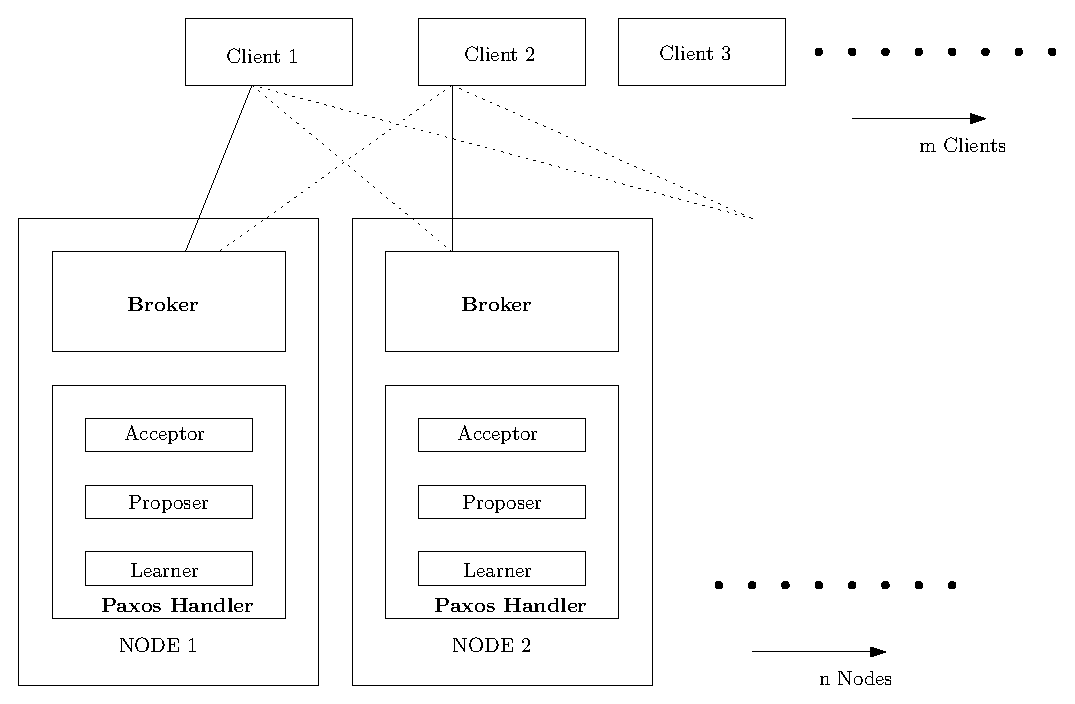
\includegraphics[width = 4.5in, keepaspectratio]{Architecture.eps}\\
\end{figure}
\subsection{Normal operation}
As seen in Section 1, during normal operation a leader simply proposes the
commands it receives, having prepared all future instances beforehand. The
leader randomly choses a majority of nodes (it is assumed that the identity of
the paxos group members is known beforehand) when trying to issue proposals.
Each node keeps a counter that represents the number of times a leader has been
elected.
We name this counter \emph{current\_proposal\_number}. 
The actual proposal number used by the leader is then calculated as $1000 * current\_proposal\_number + node\_id$, 
ensuring that proposal numbers are unique per node, and that they go
up each time a new leader is elected. Note that this assumes that there will be
less than 1000 nodes - an assumption that could easily be removed by increasing
the value of the multiplier further. As noted before, if a non-leader node's
paxos handler receives a client command, it forwards the command to the leader.
Acceptors reply to proposals with either an ``OK'' or with the highest proposal
number prepared. During normal operation, acceptors will always reply to
proposals with ``OK''.

Each node also keeps a counter for the last run command - that is, the last
command that was executed by the state machine. The leader tries to issue
proposals in sequential order, so that values get sequentially chosen (and can
get run right away). Gaps may occur in leader failures, discussed in the next
subsection.

\subsection{Node Failures}
Node or communication failures are detected in the system when any node can't
open a transport connection to some other node. Two possible situations could happen:

\begin{enumerate}
\item Leader can't open a connection to some acceptor or learner. 
\item A non leader can't open a connection to a leader while trying to forward a command.
\end{enumerate}

The first situation is easily dealt with: the leader simply ignores the failure
and contacts another acceptor - until it gets a
majority.

The second situation means that some node can't communicate with the
leader. This could either be because the leader is down or because the
communication link is broken. In either case, the node that can't reach the
leader does a broadcast to all other nodes, in order to elect a new leader. In
our implementation, the election of leaders is deterministic and cyclical, so
that the new leader id simply the old leader id plus one (mod number of nodes).
Whenever a node gets an Elect New Leader message, it updates the leader (if it
had not done already) and increases its current\_proposal\_number by 1. This
ensures that if the older leader recovers in the future, it will always see a
proposal number promised to be greater than what it proposes and thus understand
that it is not the leader anymore. It is easy to figure out who the new leader
is, as each proposal number encodes the leader's id and current\_proposal\_number.
The new leader proceeds by preparing all future instances on a majority of
nodes, making sure accepted values in between
gaps are chosen, and proposing no-ops for gaps with no accepted values, as
illustrated in Section 1. 

\section{Limitations}
\begin{itemize}
\item For the sake of the assignment, we assumed that the number of nodes is
less than 1000. This number can be easily increased, as noted before.
\item Reconfiguration and recovery are not supported (although message failure
is).
\item Client does the error handling itself. i.e. if the there is an error in
the communication between client and a broker, the client implements the
retry/ignore logic.
\end{itemize}

\section{Running the code}
To ease the starting of the servers and brokers, we are submitting a few scripts.
\begin{itemize}
\item {\em start\_nodes.py}: Starts as many nodes (broker and paxos handlers) as given via argument. Usage:
\begin{verbatim}
start_nodes.py -l NUM_LOCKS -n NUM_NODES
\end{verbatim}
This will start a bunch of nodes as servers running on different ports on the
localhost. And will also output the port numbers for the broker and paxoshandler
on each node. After this you can just run the following commands on the client:
\begin{verbatim}
Broker-remote [-h host[:port]] Lock mutexNo ClientId
\end{verbatim}
Or
\begin{verbatim}
Broker-remote [-h host[:port]] Unlock mutexNo ClientId
\end{verbatim}
\end{itemize}

In order to demonstrate the correctnes of our implementation, we have devised a
few tests, which we will demonstrate in person:
\begin{itemize}
\item {\em test-failed-message.sh}: Script to simulate failed messages.
(Automatically calls start\_nodes.py)\\ This script starts 3 nodes and runs a
few client requests and then issues an elect new leader (similar to what a node
would do in case of message failure). 
\item {\em test-kill-leader.sh}: Script to kill a leader and see if the Paxos
nodes are still working.\\ This script starts 3 nodes and after running a few
client requests, kills the leader, then tries to run a few other commands. 
\pagebreak
\item {\em test-kill-2-leaders.sh}: Script to kill one leader after another
to see if the remaining nodes still achieve
progress.

\begin{itemize}
\item Starts 5 nodes.
\item Runs a few client requests.
\item Kills the leader.
\item Runs some more client requests.
\item Kills the second leader.
\item Runs some more client requests.
\end{itemize}

\item {\em test-kill-2-nodes.sh}: Script to kill a leader and a non-leader node,
to see if progress is still achieved. 
\begin{itemize}
\item Starts 5 nodes.
\item Runs a few client requests.
\item Kills a non-leader.
\item Runs some more client requests.
\item Kills the leader.
\item Runs some more client requests.
\end{itemize}

\item {\em test-gap.sh}: Tests the correct implementation of a new leader when
there are gaps in the instances.
\begin{itemize}
\item Starts 5 nodes. 
\item Learns values for instances 0 and 3
\item Accepts a value for instance 1 on a node.
\item Kills leader
\item (new leader should run phase 2 for instnace 1, and propose no-op for instance 2)
\item Runs some more client requests.
\end{itemize}

\end{itemize}

\end{document}
